% !TeX root = ../main.tex
\section{Communities}
\label{sec:communities}

Wir suchen Communities im Arbeitsnetz aus Kapitel~\ref{sec:reduktion}. Die
Connected Components sind dort bereits beschrieben. Neben 413 isolierten
Athleten umfasst die grösste Komponente 96,6\,\% der Athleten.

\subsection{Cliquen und k-Core}
Der innerste k-Core des Arbeitsnetzes hat k = 113 und umfasst 114 Athleten
aus 71 Nationen. Alle 114 sind an denselben zwei Tagen der Weltmeisterschaft
2009 in Rom erfasst. Da die Projektion alle Athleten eines Veranstaltungstags
vollständig verbindet, bilden grosse Veranstaltungen automatisch Cliquen und
dichte Kerne. Cliquen, n-Cliquen und k-Cores zeigen in unserem Modell
deshalb vor allem einzelne Veranstaltungen. Für die Suche nach Communities
verwenden wir stattdessen Verfahren, die die gesamte Netzwerkstruktur
berücksichtigen.

\subsection{Louvain und Label Propagation}
Louvain findet mit den Kantengewichten eine Modularity von Q = 0,76, also
eine ausgeprägte Community-Struktur. Neben den 413 isolierten Athleten
entstehen 60 Communities, davon 44 mit mindestens zehn Athleten.
Tabelle~\ref{tab:communities} zeigt zwei Typen. Die vier grössten
Communities enthalten zusammen 48,8\,\% der Athleten. Sie sind
international, keine Nation stellt mehr als 6\,\% der Mitglieder. Sie
unterscheiden sich vor allem zeitlich und bilden Generationen, deren
Athleten an denselben Meisterschaften starteten. C4 um die
Europameisterschaften der frühen 2000er-Jahre, C2 um die Weltmeisterschaft
2009, C3 um die Kurzbahn-WM 2014 mit Schwerpunkt Ostasien und C1 um die
aktuellen Weltmeisterschaften. Die übrigen grossen Communities sind
national oder regional, ihr häufigster Wettkampf ist meist eine nationale
Meisterschaft. Elf der 26 Communities mit mindestens 150 Athleten bestehen
zu mindestens 90\,\% aus einer Nation. Der Frauenanteil liegt in allen
Communities ab 150 Athleten zwischen 41 und 55\,\%, was zum schwachen Geschlechtereffekt
aus Kapitel~\ref{sec:reduktion} passt.

\begin{table}[H]
  \centering
  \caption{Ausgewählte Louvain-Communities im Arbeitsnetz, nummeriert nach
  Grösse. Jahrgang und Jahr: Median der Geburtsjahre und der
  Veranstaltungstage. Wettkampf: Wettkampf mit den meisten Mitgliedern.
  Eigene Auswertung.}
  \label{tab:communities}
  \small
  \begin{tabular}{@{}lrrlrrl@{}}
    \toprule
    & Athleten & Nationen & Grösste Nation & Jahrgang & Jahr & Wettkampf \\
    \midrule
    C1 & 2\,064 & 158 & Australien, GB (je 5\,\%) & 2002 & 2021 & Weltmeisterschaften \\
    C2 & 1\,881 & 135 & Südafrika (4\,\%) & 1988 & 2009 & WM 2009 Rom \\
    C3 & 1\,304 & 140 & Japan (6\,\%) & 1996 & 2015 & Kurzbahn-WM 2014 \\
    C4 & 1\,175 & 113 & Ukraine (3\,\%) & 1978 & 2001 & Europameisterschaften \\
    \midrule
    C8 & 200 & 12 & Spanien (90\,\%) & 1997 & 2018 & Spanische Meisterschaften \\
    C9 & 185 & 2 & Türkei (99\,\%) & 2002 & 2019 & Türkische Klubmeisterschaft \\
    C19 & 168 & 25 & Schweiz (60\,\%) & 2000 & 2018 & Schweizer Meisterschaften \\
    \bottomrule
  \end{tabular}
\end{table}

Abbildung~\ref{fig:communities} zeigt die vier grössten Communities im
Layout von Abbildung~\ref{fig:athletenprojektion}. Sie liegen von links
nach rechts in zeitlicher Reihenfolge: C4, C2, C3 und C1. Das Layout, das
ohne Kenntnis der Communities oder Jahrgänge berechnet wurde, ordnet die
Athleten damit entlang der Generationen an. Die übrigen, überwiegend
nationalen Communities bilden vor allem den unteren Teil des Netzes.

\begin{figure}[H]
  \centering
  {\sffamily\small Louvain-Communities (Gewicht $\geq$ 3)}\\[1ex]
  % Nur leere Bildränder ausblenden. Die ursprüngliche PNG Datei bleibt erhalten.
  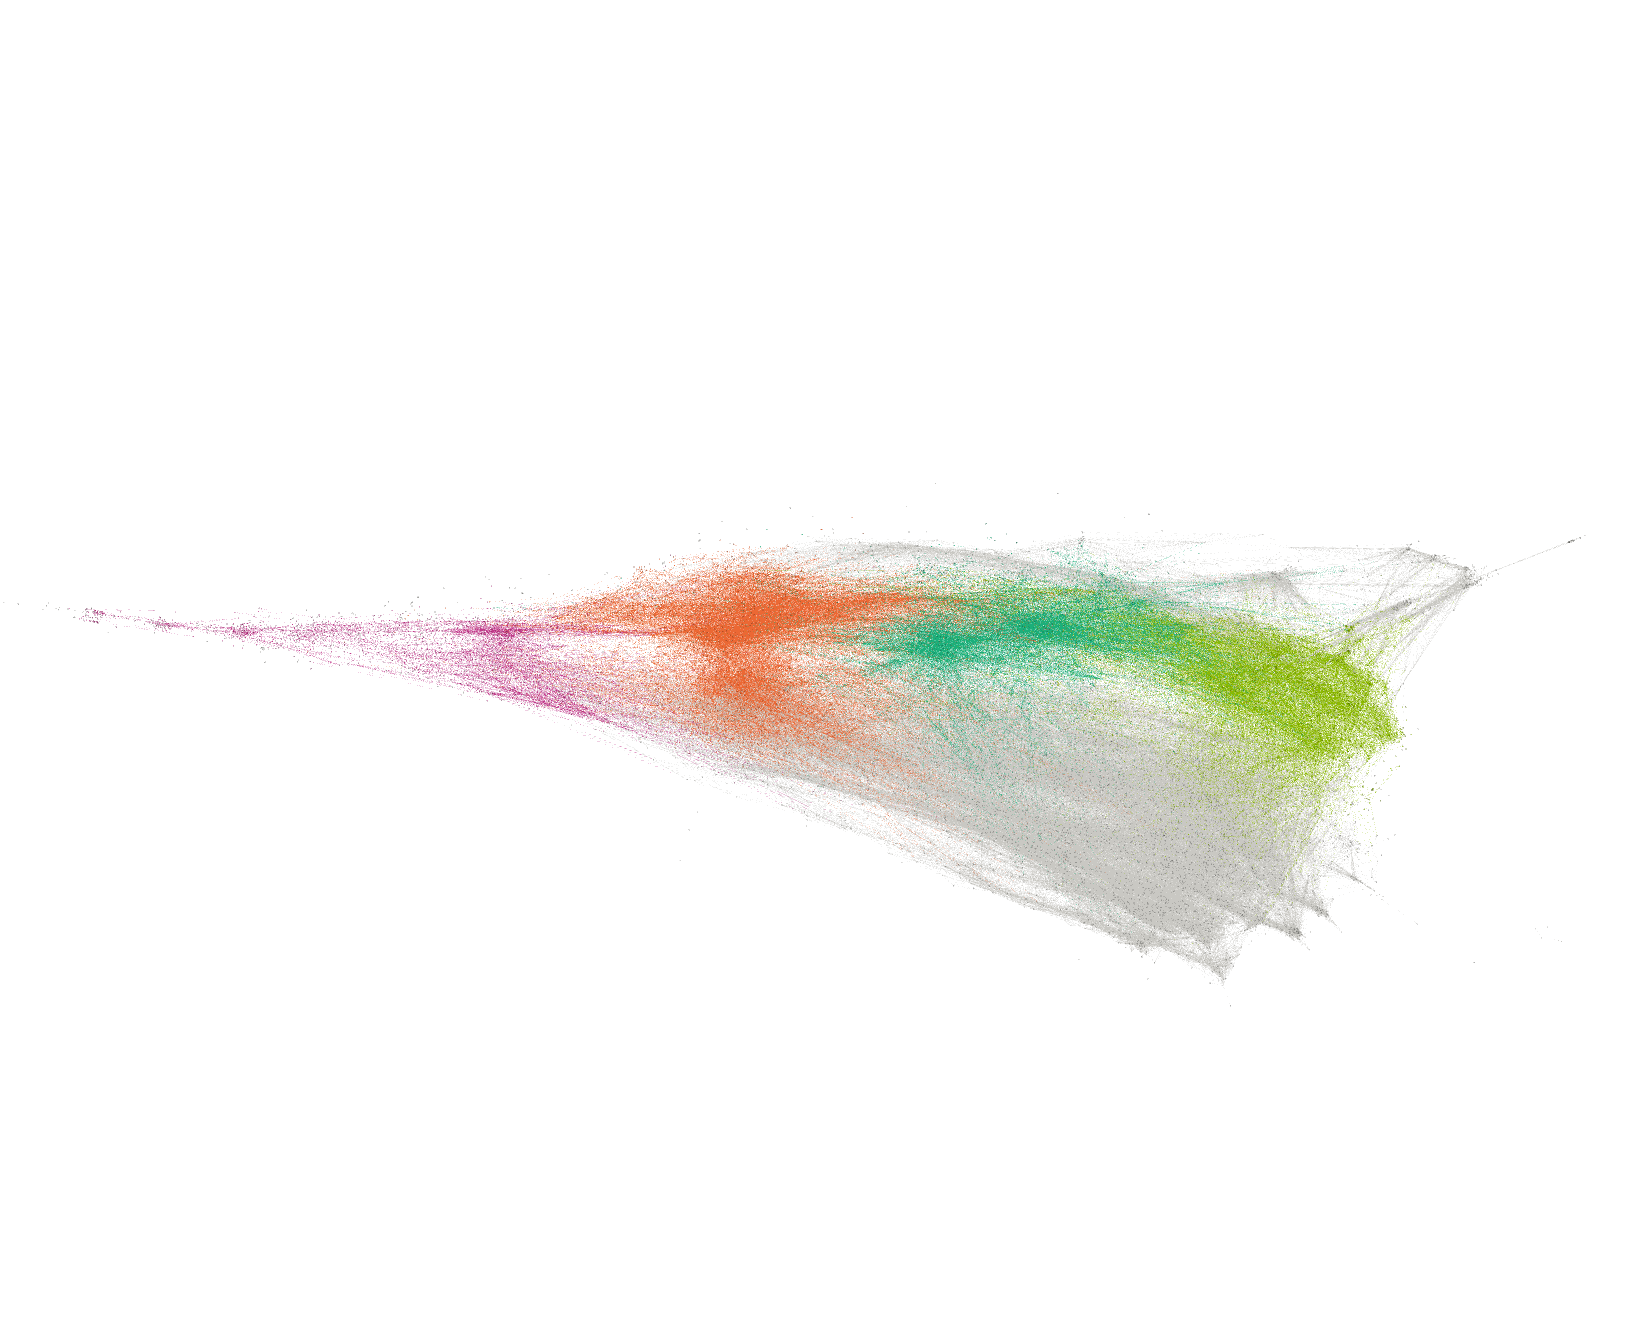
\includegraphics[width=\textwidth,trim=0 316 38 480,clip]{Athletes_Communities.png}\\[1ex]
  {\sffamily\footnotesize
  \textcolor[HTML]{C13A8A}{\Large\textbullet}~C4 (1978)\quad
  \textcolor[HTML]{EB6834}{\Large\textbullet}~C2 (1988)\quad
  \textcolor[HTML]{1BAF7A}{\Large\textbullet}~C3 (1996)\quad
  \textcolor[HTML]{8CB900}{\Large\textbullet}~C1 (2002)\quad
  \textcolor[HTML]{C9C8C3}{\Large\textbullet}~Übrige Communities}
  \caption{Athletenprojektion im Layout von
  Abbildung~\ref{fig:athletenprojektion}, gefärbt nach den vier grössten
  Louvain-Communities des Arbeitsnetzes. In Klammern der Median der
  Geburtsjahre. Eigene Darstellung in Gephi.}
  \label{fig:communities}
\end{figure}

Label Propagation dient als zweites Verfahren, da es auch für grosse Netze
geeignet ist. Girvan-Newman berechnet nach jeder entfernten Kante alle
Edge-Betweenness-Werte neu und ist für dieses Netz zu aufwendig. Label
Propagation erreicht Q = 0,73 und findet dieselbe Grobstruktur. Die
Übereinstimmung der beiden Zuordnungen beträgt 0,79 (Normalized Mutual
Information, 1 = identisch). C1 und C2 werden zu 95 bzw. 94\,\% gleich
zugeordnet. C3 und C4 teilt Label Propagation dagegen anders auf. Die
Generationen sind damit robust, ihre Grenzen aber unscharf.

Louvain findet auch in zufälligen Netzen Gruppen. Wir prüfen deshalb mit
einem Hypothesentest, ob die Modularity über das hinausgeht, was die
Gradverteilung allein erzeugt. Als Referenz dienen 100 Configuration Models
mit derselben Gradverteilung wie das Arbeitsnetz. Da diese keine Gewichte
kennen, vergleichen wir ungewichtet. Das Arbeitsnetz erreicht so
Q = 0,71, die Referenz-Netzwerke im Mittel 0,11 und höchstens 0,11. Keines
erreicht den beobachteten Wert, die Community-Struktur ist damit signifikant
($p < 0{,}01$, $\alpha = 0{,}05$).

\subsection{Communities und Nationen}
45,7\,\% der Athleten liegen in einer Community, die von ihrer eigenen
Nation dominiert wird. Im Median hat eine Nation die Hälfte ihrer Athleten
in derselben Community. Das entspricht der nationalen Prägung aus
Kapitel~\ref{sec:reduktion}: Wer vor allem national startet, bleibt in der
nationalen Community, international startende Athleten wechseln in die
Generationen. Michael Phelps gehört zu C2, der Generation um die
Weltmeisterschaft 2009. Von den 160 Schweizern liegen 101 in C19, zusammen
mit Athleten aus Zypern und Liechtenstein, 27 in C2 und 18 in C4. Dies
bestätigt die Contextual View: Die Mehrheit ist national vernetzt, die
international startenden Schweizer verteilen sich auf die Generationen.

\subsection{Communities im Nationennetz}
Im Nationennetz findet Louvain fünf Communities, darunter St.\ Kitts und
Nevis als isolierte Nation. Mit Q = 0,20 ist die Struktur schwach, was zur
hohen Density des Nationennetzes passt. Die Gruppen sind dennoch plausibel:
Europa (50 Nationen), Asien-Pazifik zusammen mit den grossen
Schwimmnationen USA, Kanada, Australien, Brasilien und Südafrika
(40 Nationen) sowie viele kleinere Schwimmnationen aus Lateinamerika,
Karibik, Afrika und dem Nahen Osten (87 Nationen). Portugal bildet mit
Angola, Mosambik und Malawi eine eigene kleine Gruppe.
